\documentclass[main.tex]{subfiles}

\begin{document}
\subsubsection{VGA-motor}
\begin{SCfigure}
    \centering
    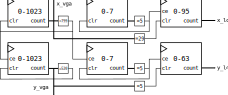
\includegraphics[width=0.85\textwidth]{vga.eps}
    \label{fig:vga}
    \caption{Räknarna inom VGA-motorn.}
\end{SCfigure}
VGA-motorns primära uppgift är att visa upp miniräknarens bildminne på
VGA-skärmen. VGA-motorn skickar färgen av en pixel åt gången, en per
klockintervall. Den börjar från det övre vänstra hörnet och går rad för rad
neråt. När pekaren når det nedre högra hörnet har det gått en sextiodels sekund
och ritningen av nästa bild påbörjas igen från det övre vänstra hörnet. För att
hålla koll på vilken pixel på skärmen som ska ritas ut används två räknare, en
för raden (\mono{y\_vga}) och en för kolumnen (\mono{x\_vga}). Utifrån
pekarens värde bestäms även hsync och vsync-signaler.

\begin{wrapfigure}{r}{0.4\textwidth}
    \vspace*{-5mm}
    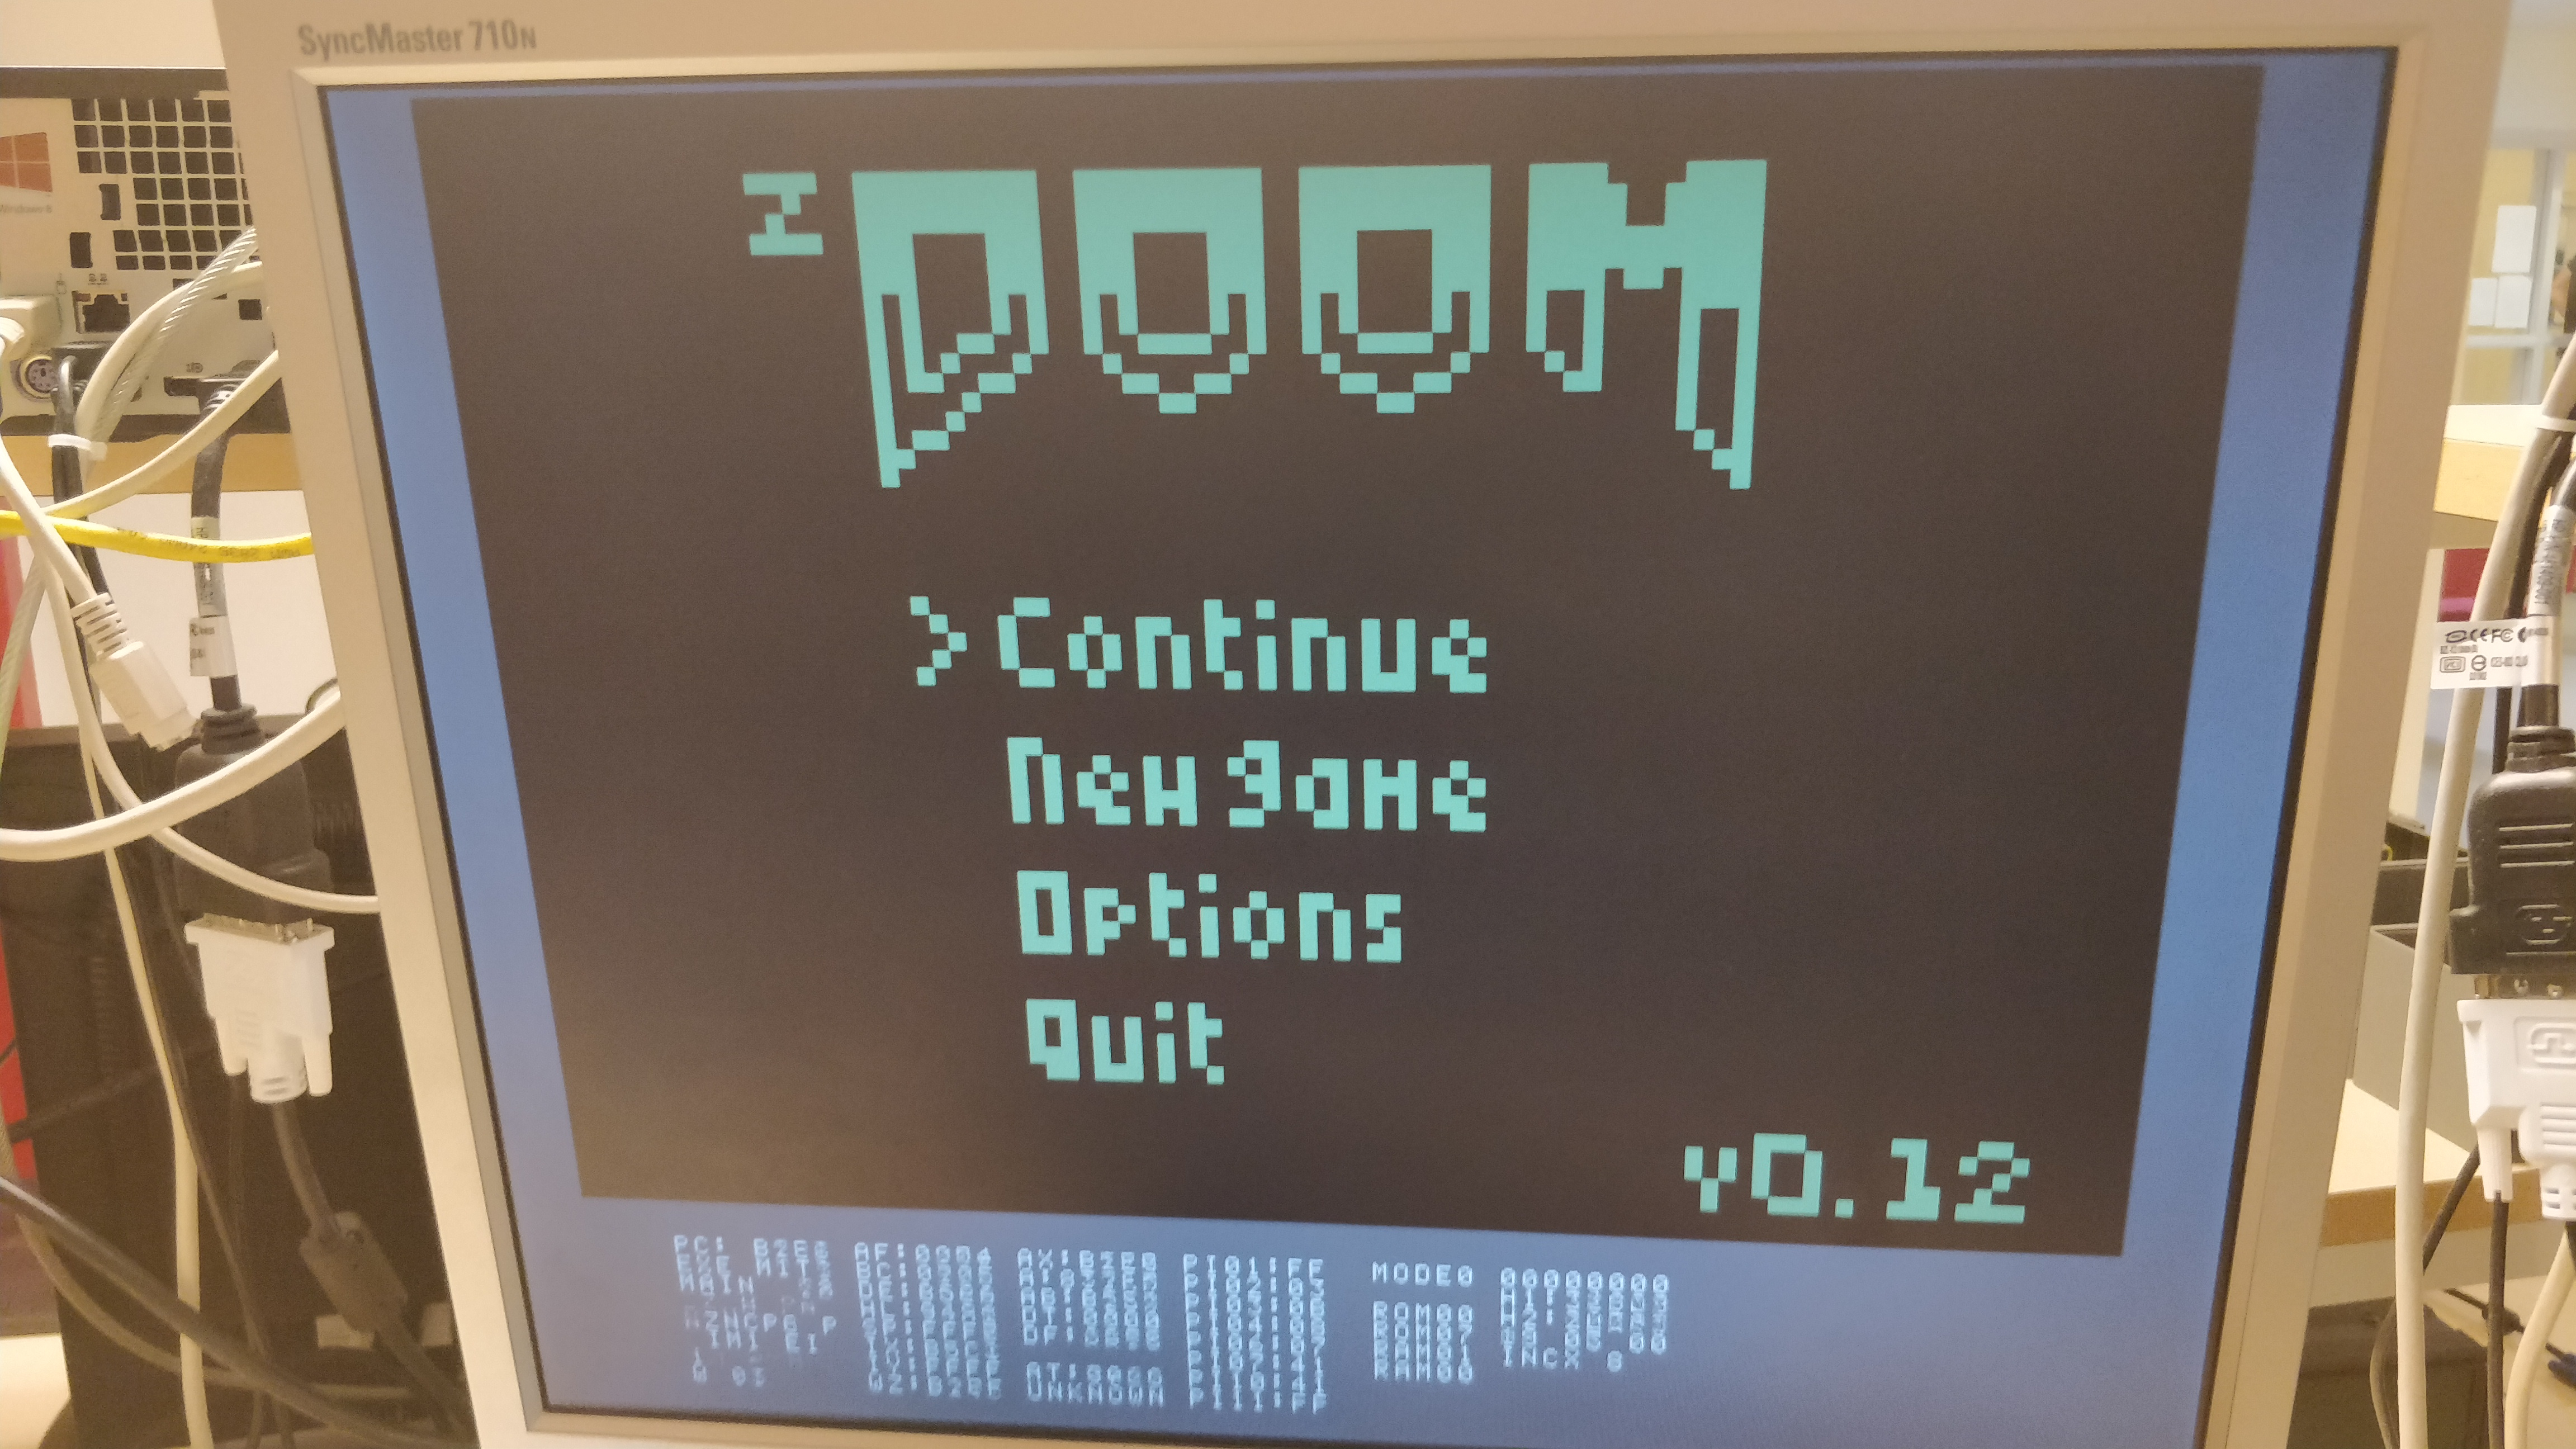
\includegraphics[width=0.4\textwidth]{monitor.eps}
    \label{fig:monitor}
    \caption{VGA-skärmens upplägg av bildminne och display för debugging samt
    blanksignal utanför bilden.}
\end{wrapfigure}
Eftersom VGA-skärmen är $640\times480$ och miniräknarens LCD-skärm är
$96\times64$ kan pixlarna i bildminnet som störst vara $6\times6$ pixlar för
att hela LCD-skärmen ska rymma. Om pixelbredden var en potens av två skulle det
vara möjligt att avgöra vilken pixel från bildminnet som skulle ritas ut
utifrån de högre bitarna i \mono{x\_vga} och \mono{y\_vga}. Eftersom
pixelbredden är sex har fyra ytterligare räknare använts. Två av räknarna (0-7)
håller koll på vilken rad och kolumn pekaren är på inom varje LCD-pixel, de
andra två (0-95, 0-63) håller koll på vilken LCD-pixel pekaren är på.
Bildminnesräknarna räknar på pixelräknarnas \mono{clr}-signal och räknar därmed
endast upp var sjätte pixel på VGA-skärmen.

Bildens position på skärmen ligger vågrätt centrerad sex pixlar från övre kant.
För att bildminnesräknarna ska hamna i fas nollställs \mono{x\_lcd} då
\mono{x\_vga} är 29 och \mono{y\_lcd} när \mono{y\_vga} är 5. För att
pixelräknarna ska hamna i fas nollställs de vid \mono{x\_clr} och
\mono{y\_clr}.

VGA-motorn visar även upp en display för debugging. Då skickas \mono{x\_vga}
och \mono{y\_vga} till en komponent som har tillgång till alla debug-signaler
som ska visas. Med hjälp av ett statiskt minne av karaktärer bestäms om pixeln
ska vara på eller av utifrån pekarens värde och värdena kan på så sätt
uttryckas med siffror och bokstäver.

\end{document}
